% architecture overview

\chapter{Overview of \CTOS{} Framework}
\label{chap:overview}

In this section, we describe the main ideas behind deep
specifications and show why they work more naturally with
abstraction layers than with regular software modules.

\section{Shallow vs. deep specifications}
%\paragraph{Deep vs. shallow specifications} 
We introduce shallow and deep specifications to describe different
classes of requirements on software and hardware components.  Type
information and program contracts are examples of ``shallow''
specifications. Type-based module interfaces (e.g., ML signatures) are
introduced to support compositional static type checking and separate
compilation: a module $M$ can be typechecked based on its import
interface $L_1$ (without looking at $L_1$'s implementation), and shown to
have types specified in its export interface $L_2$.

To support compositional verification of strong functional correctness
properties on a large system, we would hope that all of its components
are given ``deep'' specifications.  A module $M$ will be verified based on
its import interface $L_1$ (without looking at $L_1$'s
implementation), and shown to {\em implement} its export interface 
$L_2$.

To achieve true modularity, we would like to reason about the
behaviors of $M$ {\bf solely} based on its import interface $L_1$; and
we would also like its export interface $L_2$ to describe the full
functionality of $M$ while omitting the implementation details.

%A desirable property for abstraction over deep specification
%is to have {\bf implementation independence}: 
%Abstraction over deep specification must satisfy the following
%{\bf implementation independence} property: 

More formally, a deep specification captures everything we want to know
about any of its implementations---it must satisfy the following
important ``implementation independence'' property:

\begin{center}
\vspace*{-.2ex}
\fbox{\parbox{.9\columnwidth}{
{\bf Implementation independence:}~~
{\em Any two implementations (e.g., $M_1$ and $M_2$) of the same deep
  specification (e.g., $L$) should have {\em contextually equivalent}
  behaviors}.}}
\vspace*{-.2ex}
\end{center}%

\noindent{}Different languages may define such contextual equivalence relation
differently, but regardless, we want that, given any {\em
  whole-program} client $P$ built on top of $L$, running
$P\oplus{}M_1$ (i.e., $P$ linked with $M_1$) should lead to the same
observable result as running $P\oplus{}M_2$.

Without implementation independence, running $P\oplus{}M_1$ and
$P\oplus{}M_2$ may yield different observable results, so we can prove
a specific whole-program property that holds on $P\oplus{}M_1$ but not on
$P\oplus{}M_2$---such whole-program property cannot be proved based
on the program $P$ and the specification $L$ alone. 

Hoare-style partial correctness specifications are rarely
deep specifications since they fail to satisfy implementation
independence. Given two implementations of a partial correctness
specification for a factorial function, one can return the correct
factorial number and another can just go into infinite loop.  A
program built on top of such specification may not be reasoned about 
based on the specification alone, instead, we have to peek into the actual
implementation in order to prove certain properties (e.g.,
termination).

%%%%%%%%%%%%%%%%%%%%%%%%%%%%%%%%%%%%%%%%%%%%%%%%%%%%%%%%%%%%%%%%
\begin{figure}[t]\scriptsize
$$
\begin{array}{l|l}
\hspace*{-2ex} 
\begin{array}[t]{l}
\verb+typedef enum {+\\
\verb+  TD_READY, TD_RUN,+\\
\verb+  TD_SLEEP, TD_DEAD+\\
\verb+} td_state;+\\
\verb++\\
\verb+struct tcb {+\\
\verb+  td_state tds;+\\
\verb+  struct tcb *prev, *next;+\\
\verb+};+\\
\verb++\\
\verb+struct tdq {+\\
\verb+  struct tcb *head, *tail;+\\
\verb+};+\\
\verb+// +\nu_\textsf{tcbp}\text{ and } \nu_\textsf{tdqp}\\
\verb+struct tcb tcbp[64];+\\
\verb+struct tdq tdqp[64];+\\
\verb+// + \kappa_\textsf{dequeue}\\
\verb+struct tcb *+\\
\verb+dequeue(struct tdq *q){+\\
\verb+  struct tcb *head,*next;+\\
\verb+  struct tcb *pid=null;+\\
\verb+  if(q == null)+\\
\verb+    return pid;+\\
\verb+  else {+\\
\verb+    head = q -> head;+\\
\verb+    if (head == null)+\\
\verb+     return pid;+\\
\verb+    else {+\\
\verb+     pid = head;+\\
\verb+     next = head -> next;+\\
\verb+     if(next == null) {+\\
\verb+      q -> head = null;+\\
\verb+      q -> tail = null;+\\
\verb+     } else {+\\
\verb+      next -> prev = null;+\\
\verb+      q -> head = next;+\\
\verb+     }+\\
\verb+    }+\\
\verb+  }+\\
\verb+  return pid;+\\
\verb+} ...+\\
\end{array}
&
\begin{array}[t]{l}
\verb+Inductive td_state :=+\\
\verb+| TD_READY | TD_RUN+\\
\verb+| TD_SLEEP | TD_DEAD.+\\
\verb++\\
\verb++\\
\verb+Inductive tcb :=+\\
\verb+| TCBUndef+\\
\verb+| TCBV (tds: td_state)+\\
\verb+       (prev next: Z)+\\
\verb++\\
\verb+Inductive tdq :=+\\
\verb+| TDQUndef+\\
\verb+| TDQV (head tail: Z)+\\
\verb++\\
\verb+Record abs:={tcbp:ZMap.t tcb;+\\
\verb+             tdqp:ZMap.t tdq}+\\
\\
\verb+Function + \hat{\sigma}_\textsf{dequeue} \verb+ a i :=+\\ 
\verb+match (a.tdqp i) with+\\
\verb+|TDQUndef => None+\\
\verb+|TDQV h t =>+\\
\verb+ if zeq h 0 then+\\
\verb+  Some (a, 0)+\\
\verb+ else+\\
\verb+ match a.tcbp h with+\\
\verb+ |TCBUndef => None+\\
\verb+ |TCBV _ _ n =>+\\
\verb+  if zeq n 0 then+\\
\verb+  let q':=(TDQV 0 0) in+\\
\verb+   Some (set_tdq a i q', h)+\\
\verb+  else+\\ 
\verb+  match a.tcbp n with+\\
\verb+  |TCBUndef => None+\\
\verb+  |TCBV s' _ n' =>+\\
\verb+   let q':=(TDQV n t) in+\\
\verb+   let a':=set_tdq a i q' in+\\
\verb+   let b:=(TCBV s' 0 n') in+\\
\verb+    Some (set_tcb a' n b, h)+\\
\verb+  end+\\
\verb+ end+\\
\verb+end ...+
\end{array}
\end{array}
$$ 
\caption{Concrete (in C) vs. abstract (in Coq) thread queues}
\label{fig:queue}
\end{figure}
%%%%%%%%%%%%%%%%%%%%%%%%%%%%%%%%%%%%%%%%%%%%%%%%%%%%%%%%%%%%%%%%
\begin{figure}[t]\scriptsize
$$
\begin{array}{l|l}
\hspace*{-2ex} 
\begin{array}[t]{l}
\verb+Definition tcb := td_state.+\\
\verb++\\
\verb+Definition tdq := List Z.+\\
\verb++\\
\verb+Record abs':={tcbp:ZMap.t tcb;+\\
\verb+              tdqp:ZMap.t tdq}+\\
\end{array}
&
\begin{array}[t]{l}
\verb+Function + \hat{\sigma}_\textsf{dequeue}' \verb+ a i :=+\\ 
\verb+match (a.tdqp i) with+\\
\verb+| h :: q' =>+\\
\verb+  Some(set_tdq a i q', h)+\\
\verb+| nil => None+\\
\verb+end ......+\\
\end{array}
\end{array}
$$ 
\caption{A more abstract queue (in Coq)}
\label{fig:queue2}
\end{figure}
%%%%%%%%%%%%%%%%%%%%%%%%%%%%%%%%%%%%%%%%%%%%%%%%%%%%%%%%%%%%%%%%

In the rest of this paper, following CompCert~\cite{Leroy-backend}, we
will focus on languages whose semantics are {\em
  deterministic} relative to external events (formally, these
languages are defined as both {\em receptive} and {\em
  determinate}~\cite{sevcik13} and they support external
nondeterminism such as I/O and concurrency by making events explicit 
in the execution traces).
Likewise, we only consider interfaces whose primitives
have deterministic specifications. If $L$ is a deterministic interface, 
and both $M_1$ and $M_2$ implement $L$, then $P\oplus{}M_1$ and $P\oplus{}M_2$
should have identical behaviors since they both follow the semantics
of running $P$ over $L$, which is deterministic. Deterministic 
specifications are thus also deep specifications.

Deep specifications can, of course, also be nondeterministic. They may
contain resource bounds~\cite{veristack}, numerical
uncertainties~\cite{chaudhuri10}, etc. Such nondeterminism should
be unobservable in the semantics of a {\em whole} program,
allowing implementation independence to still hold.  We leave the
investigation of nondeterministic deep specifications as future work.


\section{Layers vs. modules} 
%\paragraph{Layers vs. modules} 
When a module (or a software component)
implements an interface with a shallow specification, 
we often hide its private memory state completely
from its client code. In doing so, we can guarantee that the client
cannot possibly break any invariants imposed on the private state
in the module implementation.

%%%%%%%%%%%%%%%%%%%%%%%%%%%%%%%%%%%%%%%%%%%%%%%%%%%%%%%%%%%%%%%%
\begin{figure}[t]
\begin{center}
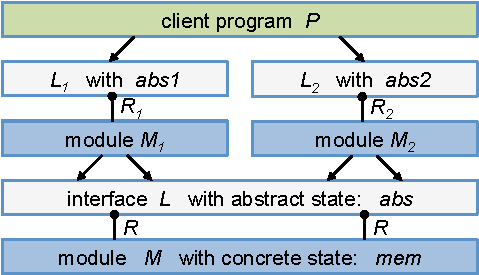
\includegraphics[scale=.7]{figs/conflict}
\caption{Client code with conflicting abstract states?}
\label{fig:conflict}
\end{center}
\end{figure}
%%%%%%%%%%%%%%%%%%%%%%%%%%%%%%%%%%%%%%%%%%%%%%%%%%%%%%%%%%%%%%%%

If a module implements an interface with a deep specification, we
would still hide the private memory state from its client, but we also
need to introduce an {\em abstract state} to specify
the full functionality of each primitive in the interface. 

For example, Fig.~\ref{fig:queue} shows the implementation of a
concrete thread queue module (in C) and its interface with a deep
specification (in Coq). The local state of the C implementation
consists of 64 thread queues (%
% e.g., a ready queue and many sleep queues, denoted as 
\textsf{tdqp}) and 64 thread control blocks
(\textsf{tcbp}).  Each thread control block consists of the thread state,
and a pair of pointers (\textsf{prev} and \textsf{next}) indicating which
linked-list queue it belongs to. The \textsf{dequeue} function 
takes a pointer to a queue; it returns the head block if the queue
is not empty, or null if the queue is empty.

In the Coq specification (Fig.~\ref{fig:queue} right; we omitted some
invariants to make it more readable), we introduce an abstract state
of type \textsf{abs} where we represent each C array as a Coq finite map
(\textsf{ZMap.t}), and each pointer as an integer index (\textsf{Z}) to the
\textsf{tdq} or \textsf{tcb} array. The \textsf{dequeue} primitive 
$\hat{\sigma}_\textsf{dequeue}$ is
a mathematical function of type $\textsf{abs} \rightarrow \textsf{Z}
\rightarrow \textsf{option (abs}\times \textsf{Z)}$; when the function returns
\textsf{None}, it means that the abstract primitive faults.  This
\textsf{dequeue} specification is intentionally made very similar to the C
function, so we can easily show that the C module indeed {\em
  implements} the specification. 

We define that a module implements a specification if there is a
{\em forward simulation}~\cite{Lynch95} from the module implementation to its
specification. In the context of determinate and receptive 
languages~\cite{sevcik13,Leroy-backend},
if the specification is also deterministic, it is sufficient to find
a forward simulation from the specification to its
implementation (this is often easier to prove in practice). 

In the rest of this paper, following CompCert, we often call the
forward simulation from the implementation to its specification
as {\em upward (forward) simulation} and the one from the specification
to its implementation as {\em downward (forward) simulation}.

Fig.~\ref{fig:queue2} shows a more abstract specification of the same
queue implementation where the new abstract state \textsf{abs'} omits
the \textsf{prev} and \textsf{next} links in \textsf{tcb} and treats each
queue simply as a Coq list. The \textsf{dequeue} specification 
$\hat{\sigma}_\textsf{dequeue}'$ is now
even simpler, which makes it easier to reason about its client,
but it is now harder to prove that the C module
implements this more abstract specification.  This explains why we
often introduce less abstract specifications (e.g.,
the one in Fig.~\ref{fig:queue}) as intermediate steps, so a
complex abstraction can be decomposed into several more tractable
abstraction steps.

Deep specification brings out an interesting {\bf new challenge}
shown in Fig.~\ref{fig:conflict}: {\em what if a program $P$ attempts to
call primitives defined in two different interfaces $L_1$ and $L_2$,
which may export two conflicting views (i.e., abstract states
\textsf{abs1} and \textsf{abs2}) of the same abstract state \textsf{abs}
(thus also the same concrete memory state \textsf{mem})?}

Here we assume that modules $M, M_1, M_2$ implement interfaces $L,
L_1, L_2$ via some simulation relations $R, R_1, R_2$ (lines marked
with a dot on one end) respectively. Clearly, calling primitives in
$L_2$ may violate the invariants imposed in $L_1$, and vice versa,
so $L_1$ and $L_2$ are breaking each other's abstraction when we run
$P$. In fact, even without $M_2$ and $L_2$, if we allow $P$ to
directly call primitives in $L$, similar violation of $L_1$ invariants
can also occur.

This means that we must prohibit client programs such as $P$ above,
and each deep specification must state the clear assumptions about its
valid client contexts. Each interface should come with a single
abstract state (\textsf{abs}) used by its primitives; and its client can
only access the same \textsf{abs} throughout its execution. 

This is what {\em abstraction layers} are designed for and why they
are more compositional (with respect to deep specification)
than regular modules! Layers are introduced to limit 
interaction among different modules: only modules with identical
state views (i.e., $R_1, R_2$ and \textsf{abs1},
\textsf{abs2} must be identical) can be composed horizontally.
 
A layer interface seems to be defining a new ``abstract machine''
because it only supports client programs with a particular view of the
memory state. The correctness of a certified layer implementation
allows us to transfer formal reasoning (of client programs) on one
abstract machine (the overlay) to another (the underlay).  

Programming with certified abstraction layers enables a disciplined way of
composing a large number of components in a complex system. Without
using layers, we may have to consider arbitrary module interaction or
dependencies: an invariant held in one function can be easily broken
when it calls a function defined in another module. A layered approach
aims to sort and isolate all components based on a carefully designed
set of abstraction levels so we can reason about one small abstraction
step at a time and eliminate most unwanted interaction and dependencies.